\documentclass[12pt]{report}
\usepackage[margin=1in]{geometry}
\usepackage{multicol}
\usepackage{caption}
\usepackage{subcaption}
\usepackage{graphicx}
\usepackage{float}
\usepackage{epstopdf}
\usepackage{setspace}
\usepackage{abstract}
%\usepackage{grffile}
\usepackage{pdfpages}
\usepackage{lscape}
\usepackage{authblk}
\usepackage{hyperref}


%Graphics Path
\graphicspath{{./MCINTOSH_Images/}{./WILEY_Images/}{./KIRBY_Images}{./WESLEY_Images}{./IANNUCCI_Images}{./BLUM_Images}{./REGAN_Images}}

\usepackage{fancyhdr}
	\pagestyle{fancy}
	\fancyhead[L]{\today}
	\fancyfoot{}
	\fancyhead[C]{OCE 496 Section 2}
	\fancyhead[R]{\thepage}


\title{\vspace{-5mm}
	\fontsize{20pt}{10pt}\selectfont
	Embedded Wireless Sensor Design for Long Term Structural Health Monitoring
}
		
\author[2]{Christopher Bessin}	
\author[1]{Patrick Blum}
\author[1]{Matthew P. Iannucci}
\author[1]{Jordan T. Kirby}
\author[1]{Zachary McIntosh}
\author[2]{Elizabeth L. Paul}
\author[1]{Michael A. Regan}
\author[2]{Justin W. Skenyon}
\author[1]{Charles J. Wesley}
\author[1]{Samuel D. Wiley}

\affil[1]{Finite Element Modelling}
\affil[2]{Instrumentation Development}
\date{\normalsize\vspace{-3mm}\today}



\begin{document}
\maketitle

%Signature Block

\textit{I have read this paper in its entirety and approve it for submission.}
\vspace{1.5cm}

\noindent\begin{tabular}{ll}
\makebox[2.5in]{\hrulefill} & \makebox[2.5in]{\hrulefill}\\
Christopher Bessin & Date\\[4ex]% adds space between the two sets of signatures
\makebox[2.5in]{\hrulefill} & \makebox[2.5in]{\hrulefill}\\
Patrick Blum & Date\\[4ex]
\makebox[2.5in]{\hrulefill} & \makebox[2.5in]{\hrulefill}\\
Matthew P. Iannucci & Date\\[4ex]
\makebox[2.5in]{\hrulefill} & \makebox[2.5in]{\hrulefill}\\
Jordan T. Kirby & Date\\[4ex]
\makebox[2.5in]{\hrulefill} & \makebox[2.5in]{\hrulefill}\\
Zachary McIntosh & Date\\[4ex]
\makebox[2.5in]{\hrulefill} & \makebox[2.5in]{\hrulefill}\\
Elizabeth L. Paul & Date\\[4ex]
\makebox[2.5in]{\hrulefill} & \makebox[2.5in]{\hrulefill}\\
Michael A. Regan & Date\\[4ex]
\makebox[2.5in]{\hrulefill} & \makebox[2.5in]{\hrulefill}\\
Justin W. Skenyon & Date\\[4ex]
\makebox[2.5in]{\hrulefill} & \makebox[2.5in]{\hrulefill}\\
Charles J. Wesley & Date\\[4ex]
\makebox[2.5in]{\hrulefill} & \makebox[2.5in]{\hrulefill}\\
Samuel D. Wiley & Date\\[4ex]
\end{tabular}

\tableofcontents
\listoffigures
\listoftables

\chapter{Introduction}
	\section{Objectives}
		\subsection{Phase One}
		\subsection{Phase Two}
	\section{Layout}
\chapter{Finite Element Model (FEM)}
	\section{Introduction}
		\subsection{Background of Claiborne Pell Bridge}
		\subsection{Introduction of FEM}
	\section{Abaqus FEM Verification}
		\subsection{L Beam Analysis}
	\section{Claiborne Pell Bridge Model}
		\subsection{Modeling Large Suspension Bridges}
		\subsection{Model Process}
		\subsection{Limitations of Abaqus FEM}

\chapter{Instrumentation Package}
	\section{Introduction}
	\section{Microprocessor}
		\subsection{Necessary Specifications}
		\subsection{Platform Options}
		\subsection{Final Platform}
	\section{Sensors}
		\subsection{Accelerometer}
			\subsubsection{Necessary Specifications}
			\subsubsection{Sensor Options}
			\subsubsection{Sensor Selection}
		\subsection{Strain Gauge}
			\subsubsection{Necessary Specifications}
			\subsubsection{Sensor Options}
			\subsubsection{Sensor Selection}
		\subsection{GPS Receiver}			
			\subsubsection{Necessary Specifications}
			\subsubsection{Sensor Options}
			\subsubsection{Sensor Selection}
		\subsection{CORS}
		\subsection{Analog to Digital Converter}
			\subsubsection{Necessary Specifications}					
			\subsubsection{Platform Options}
	\section{Electronics Design}
			\subsection{Introduction}
\indent The unique requirements for the sensor developed for deployment on the Claiborn Pell Newport Bridge set the sensor apart from off-the-shelf sensors readily available for purchase.
The sensor package needed to record high precision, high resolution accelerometer and strain gauge data continuously for an extended period of time. 
The longevity of the package was dependent upon the battery capacity and data storage capacity. 
This could have been solved by utilizing a large bank of batteries and multiple hard disk drives; however it was determined that this was a not a feasible option. 
Instead the sensor package would scavenge energy to recharge batteries and transmit data to a base station wirelessly. 
The addition of these two requirements greatly increased the complexity of the sensor package design. \\

\indent 

\subsection{Circuitry}

\subsubsection{Voltage Regulation}
The voltage input for most systems on the sensor board are a range of voltages between 3.3V-5V.
This posed a basic issue due to the output voltage of the 12V battery. 
The solution was to use two LM317 linear voltage regulators.
It was initially proposed to use the two regulators in series, such that the voltage dropped from 12V to 5V and then to 3.3V.
However, due to the current rating on the devices, it was decided to use the regulators in parallel and drop the voltage from 12V to 5V and 12V to 3.3V.
The complete circuit may be found in Figure \ref{fig:Schematic_VoltageReg}.
The LM317 technical specifications are displayed in Table \ref{tab:LM317} 

\begin{table}[h]
\centering
\begin{tabular}{|l|c|}
\hline
\textbf{Parameter} & \textbf{Value}\\
\hline
Input Voltage Differential ($V_{in}-V_{out}$)& 3V $\le V_{in}-V_{out} \le$ 40V\\
Output Voltage ($V_{out}$) & 1.2V $\le V_{out} \le$ 37V\\
Output Current ($I_{out}$) & 1.5A\\
Max Power Dissipation ($P_{D}$) & 20W\\
Package Type				   & TO-220\\
\hline
\end{tabular}
\caption{LM317 Adjustable Linear Regulator Specifications}
\label{tab:LM317}
\end{table}

The output voltage can be set using Equation \ref{eqn:LM317} where $R_1= 240\Omega$ and $I_{adj}\le 100\mu A$.
It should be noted the $V$ is not the input voltage, but a unit placeholder.
Since $I_{adj}$ is very low, the error associated with it is almost negligible. 
\begin{equation}
V_{out} = 1.25V(1+\frac{R_2}{R_1}) + I_{adj}R_2
\label{eqn:LM317}
\end{equation}
The regulation circuit was tested using a 7.7Ah 12V battery in order to confirm the output voltages. %Possibly test and record range of input and output voltages
The voltages recorded were steady at approximately 3.5V and 5.3V.
The error is believed to be due to the inherent tolerance in the passive components used in the circuit.
Also in field use, the package will be subject to a wide range of temperatures that will cause the error in voltage to vary.

\subsubsection{ADC Impedance Matching}
\label{sec:ADC_Impedance_Matching}
As mentioned in Section \ref{sec:ADC_Impedance_Issues}, impedance matching issues were encountered when sampling accelerometer data with the micro-controller.
To avoid such issues in the final design, an impedance matching op-amp was used.
The MCP606 op-amp was used due to its rail-to-rail output, low input offset voltage, unity gain stability and low power characteristics. 
In order to act as a buffer for the input of the ADC, the op-amp was configured as in Figure \ref{fig:op-amp_standard}; where $R_1$ and $R_2$ are governed by the Equation \ref{eqn:op-amp_gain}. 
Since the op-amp will be used with unity gain (gain = 1) then both resistors are $0\Omega$ and just wired connections \cite{ArtofElectronics}.

\begin{figure}
\centering
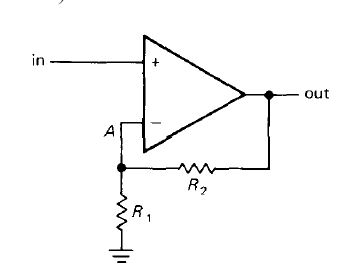
\includegraphics[scale=1]{Op-Amp_Standard}
\caption{Standard configuration of op-amp as a buffer}
\label{fig:op-amp_standard}
\end{figure}

\begin{equation}
gain = 1 + \frac{R_{2}}{R_{1}}
\label{eqn:op-amp_gain}
\end{equation}

\subsubsection{Decoupling Capacitors}
In order to reduce noise on the power supply line to each component, decoupling capacitors were added to each device between the voltage input and ground.
Decoupling capacitors act as low-pass filters, thus removing high frequency voltage differentials.
To ensure no inductance due to the transmission length between the decoupling capacitors and device inputs, the transmission length was minimized \cite{ArtofElectronics}.


\subsection{Printed Circuit Board}
\label{sec:PCB}
In order to combine the system in an efficient manor, it was decided that a printed circuit board (PCB) must be designed to carry the components.
This would make future sensor packages easy to manufacture for additional sensor nodes on the bridge and ensures consistency between packages.
It should be noted that all schematics and circuit board files were created using National Instruments Multisim 13.0 and Ultiboard 13.0 respectfully.
All schematics and board files may be found at \url{https://github.com/mpiannucci/SeniorDesign/tree/master/hardware}.
 
\subsubsection{Requirements for PCB}
Initially the requirements for the PCB were to create a carrier board that would allow for the addition and removal of package components via header sockets.
This would allow for the purchase of many off-the-shelf components that would be able to be installed with minimal effort.
For various reasons, the scope of the PCB was change from being a carrier board to completely integrating all of the components.
This posed difficulties as many of the components utilized in the package were bought as standalone solutions with dedicated PCBs for each component.
As a solution for this, all component that shipped with PCBs had all of their circuitry mimicked on the main PCB.
This holds true for all components except for three; BeagleBone Black, Trimble Copernicus II GPS receiver and the XBee Pro S3B wireless receiver.
It was decided that it was more appropriate to create sockets for each of these components to plug into for specific reasons.
Although the board files for the BeagleBone Black are readily available to download, it was deemed unnecessary to recreate the board.
For the Trimble Copernicus II GPS receiver, it was decided that because of the sensitivity in the design of the antenna circuit that it would be best to use the off-the-shelf board.
The board purchased has the antenna circuit integrated with impedance matched SMA connector for the antenna.
Due to unforeseen issues with interfacing the XBee Pro S3B wireless receivers, the receiver was not incorporated in the initial version of the system design.
Section \ref{sec:XBeeFuture} discusses the future work to be done with the XBee Pro S3B receivers.

\subsubsection{Progress on Printed Circuit Board}
All component footprints for components in the sensor package were created in Multisim 13.0 and Ultiboard 13.0.
The library of components may be found at \url{https://github.com/mpiannucci/SeniorDesign.git} under \verb|./hardware/UsrComp_S_SHMComps.usr|.
A basic board was laid out, however trace routing was not completed due to unresolved net issues.
Although the board design was not finished, a comprehensive schematic was created and will prove useful for future development of the board.
The schematics may be found in Appendix \ref{app:Schematic}.
			
	\section{Software Design}
	\section{Package Power}
		\subsection{Power Budget}
		\subsection{Energy Scavenging Potential}
			\subsubsection{Wind Potential}
			\subsubsection{Solar Potential}
		\subsection{Battery Selection}
		
\chapter{Data Collection}
	\section{Phase One Data Collection}
		\subsection{6g Tri-Axial Accelerometer Data}
	\section{Phase Two Data Collection}
		\subsection{6g Tri-Axial Accelerometer Data}
		\subsection{1.5g Tri-Axial Accelerometer Data}
		\subsection{Cell Phone Accelerometer}
		\subsection{Battery Discharge Curve}
		\subsection{Experimental Observed Efficiency}
\chapter{Data Analysis}
	\section{Phase One Data Analysis}
		\subsection{Comparison of Preliminary Abaqus Model and Preliminary Data}
	\section{Phase Two Data Analysis}
		\subsection{Comparison of Developed Abaqus Model with Literature}
		\subsection{Comparison of Developed Abaqus Model with Developed Abaqus Model}	
		
\chapter{Future Development}
	\section{Instrumentation}
		\subsection{Integration of Strain Gauge}
			
\subsubsection{Integration of Strain Gauge}

\indent Figure \ref{fig:OmegaSoldered} is one of the 3-element rosette strain gauges with pre-soldered ribbon leads. Purchased from omega engineering with
model number SGD-6/120RYT23. These strain gauges were necessary after realizing the difficulty of soldering leads to the original set of strain gauges.
The pre-soldered ribbon leads on the second set of strain gauges also proved to be unsuccessful during experimentation. This was because the leads would
not stay secured to the attaching clips while tests were being run. Even with the persistent attempts to get the strain gauges connected and working
correctly, the data received was still very inaccurate. One possible contributing factor to this may have be the lack of precision when applying the
strain gauge to the exact location on the beam. However, one definite factor that contributed to the inaccurate data from the strain gauges was the
type of strain gauge that was used. A strain gauge with a different gauge factor and a higher resistance would have been more favorable. The higher
the resistance of a strain gauge, the higher the sensitivity. The original sets of strain gauges had a resistance of 120 $\Omega$, but to precisely
measure strain on a beam the resistance must be much higher, 350 $\Omega$ or more. The costs for a pack of 6 similar strain gauges with a
resistance of 350 $\Omega$ from omega engineering is one hundred dollars. Another factor that halted the efforts to apply the strain gauge was
that they required another ADC output. It is possible to make more outputs, however this also demands that the time synchronization is even more
accurate. Nevertheless, higher resistant strain gauges would be better for sensor packages for future developments. \\

\begin{figure}[h!]
\centering
\includegraphics[width=\textwidth]{./MCINTOSH_Images/Strain_Gauge_with_Leads.png}
\caption{Omega 3-Element Rosette with pre-soldered leads.}
\label{fig:OmegaSoldered}
\end{figure}

\subsubsection{Package Assembly}

\paragraph{Package Location}
\indent Figure \ref{fig:PackageLocation} is an Abaqus visualization of the Newport Bridge with the proposed location for the sensor package to be mounted.
As shown in the figure, the center of the bridge is the best location for the sensor package. This is because the greatest amplitude of displacement will
occur during the first mode of vibration at the middle of the bridge. Mounting the sensor package to the bridge must be done without damaging the
structure in any way. The sensor package must also be capable of being moved easily. Most importantly, the package must be secured without any of its
own motion, this is so that the sensors can recognize the movement of the bridge and not the package itself. The most economical way of securing the
sensor package to the bridge is to use powerful magnets. Neodymium Magnets are strong magnets that work well in all environments and resist
demagnetization. One negative aspect of the magnets is that it can be prone to corrosion if not protected with a coating properly. There is also a
concern that the magnetic field can disrupt the electronics within the case. However, these issues can be prevented if the correct precautions are
taken. The magnets come in many shapes and sizes, shown in Figure \ref{fig:PackageLocation} one can see that the magnets can be bought with pre
made holes for screws for mounting to the package. The magnets in figure \ref{fig:PackageLocation} are model MMR-A-XC from KJMagnetics.com. This
magnet is hardly larger than a penny, yet it can easily be screwed into the sensor package and pull a force of 54.14 pounds. With two of these
magnets screwed into the sensor package the package would be secured to the bridge. If calculations are run to prove the wind speed on the
surface of the package to be too much for this pull force, stronger magnets are available. KJMagnetics.com also has similar magnets but with
different pull forces ranging from 26.8 pounds to 260 pounds. These magnets can be used for securing the solar panels and wind turbine as
well. Figure \ref{fig:Proposed Package, Panels and Turbine Location} shows a practicable location for the sensor package along with the solar
panels above and the wind turbine hanging just below. The sensor package should be mounted on the outside of one of the major vertical beams
at midspan of the bridge. The solar panels and wind turbine must be mounted close within a reasonable distance to keep the cable length to
a minimum. The best place to mount the solar panels is on top of the upper horizontal beam on the southern side of the bridge. This will
allow for the most amount of sun light and the shortest amount of cable necessary. The best place to mount the wind turbine is on the
bottom of the lower horizontal beam on the southern side of the bridge. This location has plenty of wind because it is above the middle
of the Narragansett Bay. By mounting the sensor package, solar panels and wind turbine below the deck on the southern side of the
bridge the package will be capable of producing its own power and accurately measuring the vibrations of the bridge.


\begin{figure}[h]
\centering
\includegraphics[width=\textwidth]{./MCINTOSH_Images/Bridge_Full_.png}
\caption{Proposed Package Mounting Location.}
\label{fig:PackageLocation}
\end{figure}

\begin{figure}[h]
\centering
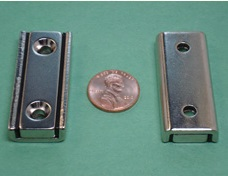
\includegraphics[width=\textwidth]{./MCINTOSH_Images/Neodymium_Mounting_Magnet.jpg}
\caption{Neodymium Mounting Magnet.}
\label{fig:Mounting Magnet}
\end{figure}

\begin{figure}[h]
\centering
\includegraphics[width=\textwidth]{./MCINTOSH_Images/Proposed_Package_Location.png}
\caption{Proposed Location for Sensor Package, Wind Turbine and Solar Panels.}
\label{fig:Proposed Package, Panels and Turbine Location}
\end{figure}


		\subsection{Wireless Transmission}
		\subsection{GPS Time Synchronization}
		\subsection{Package Assembly}
			\subsubsection{Fabrication of Circuit Board}
			\subsubsection{Battery Integration}
			\subsubsection{Package Enclosure}
			\subsubsection{Power Management}
			\subsubsection{Package Location}
	\section{FEM}
		\subsection{Model Improvements}
		\subsection{Dynamic Loading}
\chapter{Conclusion}

\appendix

\chapter{Sensor Package Schematics}
\label{app:Schematic}
\section{LM317 Adjustable Voltage Regulators}
\begin{figure}[H]
\centering
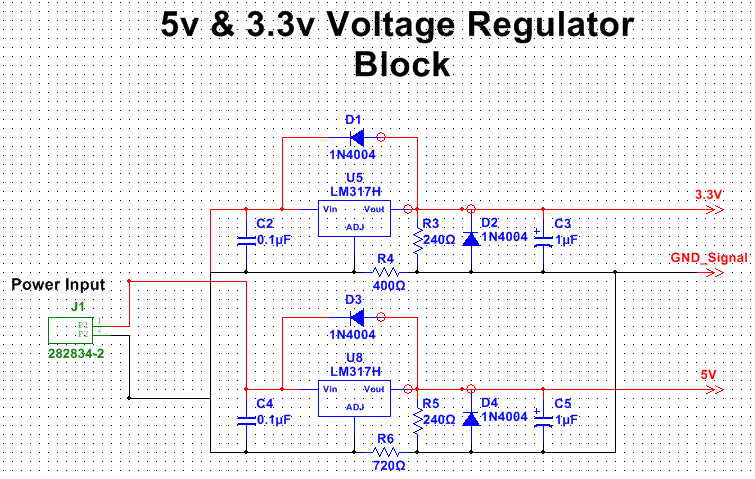
\includegraphics[width=\textwidth,height=\textheight,keepaspectratio]{./KIRBY_Images/Multisim_VoltageRegulation}
\caption{Schematic of 5V and 3.3V voltage regulator circuit}
\label{fig:Schematic_VoltageReg}
\end{figure}

\section{BeagleBone Black}
\begin{figure}[H]
\centering
\includegraphics[width=0.9\textwidth,height=0.9\textheight,keepaspectratio]{./KIRBY_Images/Multisim_BBB}
\caption{Schematic of BeagleBone Black}
\label{fig:Schematic_BBB}
\end{figure}

\section{ADS1113 Analog-Digital Converter}
\begin{figure}[H]
\centering
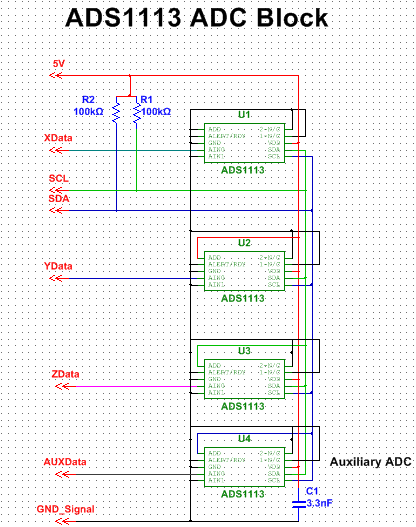
\includegraphics[width=0.9\textwidth,height=0.9\textheight,keepaspectratio]{./KIRBY_Images/Multisim_4ADC}
\caption{Schematic of four ADS1113 ADC units in parallel}
\label{fig:Schematic_ADS1113}
\end{figure}


\section{MMA7361 Accelerometer}
\begin{figure}[H]
\centering
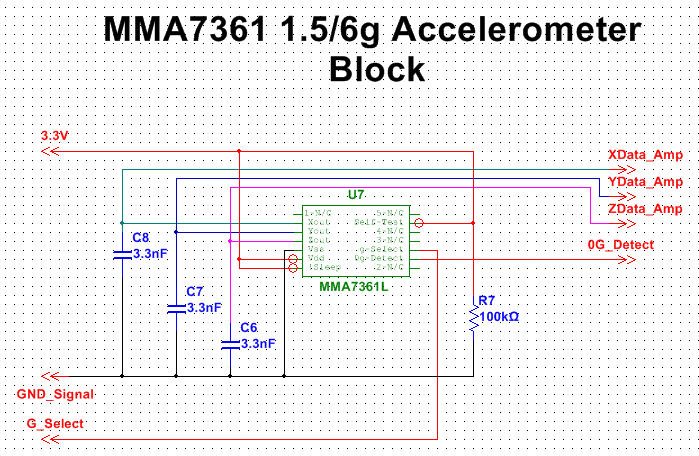
\includegraphics[width=\textwidth,height=\textheight,keepaspectratio]{./KIRBY_Images/Multisim_MMA7361}
\caption{Schematic of MMA7361 $\pm 1.5g/ \pm 6g$ Tri-Axial Accelerometer}
\label{fig:Schematic_MMA7361}
\end{figure}

\section{Trimble Copernicus II GPS Receiver}
\begin{figure}[H]
\centering
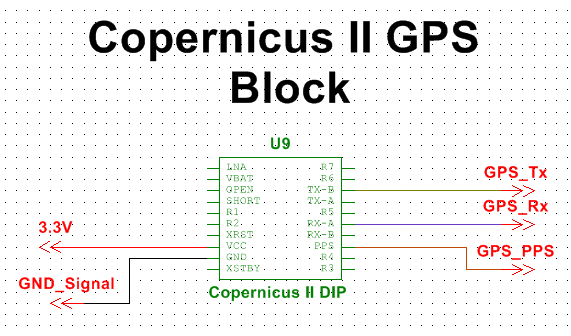
\includegraphics[width=\textwidth,height=\textheight,keepaspectratio]{./KIRBY_Images/Multisim_GPS}
\caption{Schematic of Copernicus II GPS Receiver}
\label{fig:Schematic_Copernicus}
\end{figure}
\end{document}